\documentclass[prc,amsmath,twocolumn,superscriptaddress]{revtex4}
%\bibliographystyle{prsty}
\usepackage{gensymb}
\usepackage{graphicx,color}
\usepackage{amssymb}
\usepackage{enumerate}
\usepackage{verbatim}
\usepackage{natbib}


\begin{document}

  \newcommand {\nc} {\newcommand}
  \nc {\Sec} [1] {Sec.~\ref{#1}}
  \nc {\IR} [1] {\textcolor{red}{#1}} 

\title{PHY905 Project 2 - Jacobi Algorithm}


\author{Alaina~Ross}

\date{\today}

%%%%%%%%%%%%%%%%%%%%%%%%%%%%%%%%%%%%%%%%%%%%%%%%%%%%%%%%%%%%%%%%%%%%%%%%%%%%%%%%%%%%%%%%%%%%%%%%%%%%%%%%%%%%%%%%%%%%%%%%%%%%%%%%%%%

\begin{abstract}
 \noindent {\bf Background:}% To solve a differential equation computationally the derivative is approximated and a system of linear equations is solved instead. Such systems can be solved via matrix equations and Gauss elimination. \\
\\ {\bf Purpose:} %The goal of this work is to implement various Gauss elimination algorithms and study the accuracy and performance of each when applied to a system of equations which result from the Poisson equation with a given example from electromagnetism. \\
\\ {\bf Method:} %We use a general Gauss elimination algorithm as well as two for tridiagonal matrixes and one which uses LU decomposition. We inspect the time to solution for varying matrix sizes and compare to the analytic solution to evaluate the accuracy of the algorithms. \\ 
\\ {\bf Results:} %We find the most accurate matrix size is $10^5$ and the fastest algorithm for this matrix size is the tridiagonal algorithm. \\
 \\ {\bf Conclusions:} %Our results demonstrate the importance of choosing the right algorithm for the given physical situation.
\end{abstract}


\maketitle

%%%%%%%%%%%%%%%%%%%%%%%%%%%%%%%%%%%%%%%%%%%%%%%%%%%%%%%%%%%%%%%%%%%%%%%%%%%%%%%%%%%%%%%%%%%%%%%%%
\section{introduction}
\label{intro}
For a single electron in a harmonic oscillator potential, the radial Schr{\"o}dinger equation is given by:
\begin{gather}
\frac{\hbar}{2m}\left(\frac{1}{r^2}\frac{d}{dr}r^2\frac{d}{dr}-\frac{\ell(\ell+1)}{r^2}\right)R_n(r) \notag \\
+\frac{1}{2}m\omega^2r^2 R_n(r)=E_{n\ell}R_n(r)
\end{gather}
where $R_n(r)$ are the radial wave functions, $\omega$ is the oscillator frequency, and $E_{n\ell}$ is the energy for the given quantum numbers:
\begin{equation}
E_{n\ell}=\hbar\omega\left(2n+\ell+\frac{3}{2}\right) \quad n,\ell = 0,1,2...
\end{equation}

In this work we will focus on $\ell=0$. Then making the substitution $u_n(r)=rR_n(r)$ and $\rho=\alpha/r$ where $\alpha^4=\hbar^2/mk$ and $k=m\omega^2$ gives:
\begin{equation}
-\frac{d^2}{d\rho^2}u_n(\rho)+\rho^2u_n(\rho)=\frac{2m\alpha}{\hbar^2}E_{n}u_n(\rho).
\end{equation}
Simplifying further, we can introduce the variable $\lambda$ such that:
\begin{equation}
-\frac{d^2}{d\rho^2}u_n(\rho)+\rho^2u_n(\rho)=\lambda u_n(\rho).
\end{equation}
This equation can be solved analytically to give the eigenvalues $\lambda_0=3$, $\lambda_0=7$, and $\lambda_2=11$.

If rather than one electron in the harmonic oscillator well there are two which are non-interacting, then Equation 1 becomes:
\begin{gather}
\left(-\frac{\hbar^2}{2m}\frac{d^2}{dr_1^2}-\frac{\hbar^2}{2m}\frac{d^2}{dr_2^2}+\frac{1}{2}kr_1^2 +\frac{1}{2}kr_2^2 \right)u_n(r_1,r_2) \notag \\
= E_n^{(2)}u_n(r_1,r_2)
\end{gather}
where $u_n(r_1,r_2)$ is a two-body wave function and $E_n^{(2)}$ is the two-electron energy. We introduce new coordinates, \textbf{r} and \textbf{R}, defined by:
\begin{gather}
\mathbf{r}=\mathbf{r_1}-\mathbf{r_2} \\
\mathbf{R}=\frac{1}{2}\left(\mathbf{r_1}+\mathbf{r_2}\right) 
\end{gather}
where \textbf{r} is the relative coordinate and \textbf{R} is the relative center-of-mass coordinate. This simplifies Equation 5 to:
\begin{gather}
\left(-\frac{\hbar^2}{m}\frac{d^2}{dr^2}-\frac{h^2}{4m}\frac{d^2}{dR^2} + \frac{1}{4}kr^2+kR^2\right)u_n(r,R) \notag \\
=E_n^{(2)}u_n(r,R)
\end{gather}
and allows for the both the wave function and the energy to be written in terms of a relative wave function and energy, $\psi(r)$ and $E_r$, and a center-of-mass wave function and energy, $\phi(R)$ and $E_R$:
\begin{gather}
u(r,R)=\psi(r)\phi(R) \\
E^{(2)}=E_r+E_R.
\end{gather}

This change of variables proves even more useful though when a repulsive Coulomb interaction is included as:
\begin{equation}
V(r_2,r_2)=\frac{\beta e^2}{|\mathbf{r}_1-\mathbf{r}_2|}=\frac{\beta e^2}{r}
\end{equation}
where $\beta e^2$ = 1.44 eVnm. As this potential only depends on the relative coordinate, we can look exclusively at the Schr{\"o}dinger equation for the relative wave function:
\begin{equation}
\left(-\frac{h^2}{m}\frac{d^2}{dr^2}+\frac{1}{4}kr^2+\frac{\beta e^2}{r}\right)\psi(r)=E_r\psi(r).
\end{equation}

Again we can make the substitution $\rho=r/\alpha$ where now $\alpha=\hbar^2/m\beta e^2$. In addition, we introduce the frequency $\omega_r=mk\alpha^4/4\hbar^2$, which reflects the strength of the oscillator potential, and the variable $\lambda = m\alpha^2E_r/\hbar^2$. Equation 12 then becomes:
\begin{equation}
-\frac{d^2}{d\rho^2}\psi(\rho)+w_r^2\rho^2\psi(\rho)+\frac{1}{\rho}=\lambda\psi(\rho).
\end{equation}
This equation has been solved analytically for some values of $\omega_r$ in~\cite{interact}. Of specific interest in this work is the case $\omega_r=0.05$, where the ground state eigenvalue is given by $\lambda=0.35$.

In this work we implement the Jacobi algorithm to solve the eigenvalue problems described above and study the performance characteristics and numerical accuracy for different grid and step sizes. In addition, we investigate the influence of the frequency $w_r$ on the shape of the wave functions in the interacting case. In Section~\ref{methods}, the implementation of the algorithm is described. In Section~\ref{results} the performance and accuracy of the code are analyzed. Finally, in Section~\ref{conc} we give a summary and our conclusions.

\section{methods}
\label{methods}
We first start by discretizing the functions in Equations 4 and 13 and approximating the derivatives as:
\begin{equation}
u''=\frac{u(\rho+h)-2u(\rho)+u(\rho-h)}{h^2}+O(h^2)
\end{equation}
where h is the step size. Realistically, the wave functions should be defined from $\rho=[0,\infty)$, however, numerically we define a minimum value, $\rho_0=0$, and a maximum value, $\rho_{max}$, which will determine the step size for a given number of mesh points, N, as:
\begin{equation}
h=\frac{\rho_{max}-\rho_0}{N}
\end{equation}

Using Equation 14, Equations 4 and 13 can be written as:
\begin{equation}
\left(\frac{2}{h^2}+V_i\right)u_i-\frac{1}{h^2}u_{i-1}-\frac{1}{h^2}u_{i+1}=\lambda u_i
\end{equation}
where $V_i$ is either $\rho^2$ for the non-interacting case, or $\omega_r^2\rho^2+1/\rho$ for the interacting case. The above equation is an eigenvalue problem that can be written in matrix form as:
\begin{equation}
\begin{bmatrix} \frac{2}{h^2}+V_1 & -\frac{1}{h^2} &0 \\ -\frac{1}{h^2}  & \frac{2}{h^2}+V_2 &-\frac{1}{h^2} \\ 0  & -\frac{1}{h^2}  &\frac{2}{h^2}+V_N \end{bmatrix}
\begin{bmatrix} u_0  \\ u_1\\ u_N \end{bmatrix}=\lambda \begin{bmatrix} u_0  \\ u_1\\ u_N \end{bmatrix}
\label{matrix}
\end{equation}

As an N dimensional matrix will have N eigenvalues and eigenvectors, the grid size necessarily determines the number of eigenvalues that will be produced. As we are only interested in the ground state and first two excited states, the minimum matrix size we can use is N = 3.

To begin the Jacobi algorithm we implement the vectors, $v_i$, and matrix, $\hat{a}$, using the Armadillo library~\cite{armadillo}. The main premise is to diagonalize the matrix via repeated unitary transformations, given by $\hat{a}'=\hat{S}^T\hat{a}\hat{S}$, which take the largest non-diagonal matrix element to zero each iteration. This process continues until all off diagonal elements are less than the specified tolerance and thus are essentially zero. Once the diagonalization is complete, the eigenvalues are simply the values left on the diagonal.

For the eigenvectors we choose as a starting point unit vectors given by:
\begin{equation}
v_0=\begin{bmatrix} 1  \\ 0\\ 0 \end{bmatrix}\quad v_1=\begin{bmatrix} 0  \\ 1\\ 0 \end{bmatrix}
\quad v_N=\begin{bmatrix} 0  \\ 0\\ 1 \end{bmatrix}.
\label{matrix}
\end{equation}
Then for each iteration in the diagonalization scheme, the eigenvectors will undergo the same unitary transformation as the matrix, namely $v_i'=\hat{S}v_i$. As the transformation is unitary, the orthogonality of the eigenvectors will be preserved.

If the coordinates of the matrix element to be sent to zero are given by $(k,l)$, the nonzero matrix elements of the rotation matrix, $\hat{S}$, are given by:
\begin{gather}
S_{(k,l)}=-S_{(l,k)}=-sin(\theta) \notag \\
S_{(k,k)}=S_{(l,l)}=cos(\theta) \notag \\
S_{(i,i)}=1 \quad i\neq k, i\neq l.
\end{gather}
After the transformation, the updated matrix elements of $\hat{a}'$ will be given by:
\begin{gather}
a'_{(k,l)}= \left(a_{(k,k)}-a_{(l,l)}\right)cos(\theta)sin(\theta)+a_{(k,l)}\left(cos^2(\theta)-sin^2(\theta)\right)  \notag \\
a'_{(k,k)}= a_{(k,k)}cos^2(\theta)-2a_{(k,l)}cos(\theta)sin(\theta)+a_{(l,l)}sin^2(\theta) \notag \\
a'_{(l,l)}= a_{(l,l)}cos^2(\theta)+2a_{(k,l)}cos(\theta)sin(\theta)+a_{(k,k)}sin^2(\theta) \notag \\
a'_{(i,k)}= a_{(i,k)}cos(\theta)-a_{(i,l)}sin(\theta) \quad i\neq k,l\notag \\
a'_{(i,l)}= a_{(i,l)}cos(\theta)+a_{(i,k)}sin(\theta) \quad i\neq k,l 
\end{gather}
Since $a'_{(k,l)}\equiv0$, $sin(\theta)$ and $cos(\theta)$ are determined via the expression above as:
\begin{gather}
cot(2\theta)\equiv \tau =\frac{a_{(l,l)}-a_{(k,k)}}{2a_{(k,l)}} \\
tan(\theta)=-\tau \pm \sqrt{1+\tau^2} \\
cos(\theta)=\frac{1}{\sqrt{1+tan^2(\theta)}} \\
sin(\theta) = tan(\theta)cos(\theta) 
\end{gather}
and the matrix elements are updated accordingly.

To determine the accuracy of our solutions, we define the average error as the average of the percentage differences of the first three energy eigenvalues calculated via the Jacobi algorithm, $\lambda_n^j$, as compared to their exact values, $\lambda_n$:
\begin{equation}
\epsilon_{avg}=\frac{1}{3}\left(\frac{|\lambda_0^{j}-\lambda_0|}{\lambda_0}
+\frac{|\lambda_1^{j}-\lambda_1|}{\lambda_1} +\frac{|\lambda_2^{j}-\lambda_2|}{\lambda_2} \right)
\end{equation}

\section{results}
In the following subsections we describe the results obtained first without the Coulomb interaction and then with it included. We discuss the numerical accuracy and performance of the methods and show the radial probability distributions for the interacting case.
\label{results}
\subsection{Non-interacting Case}
We first implement the Jacobi algorithm with only the harmonic oscillator potential. As stated in Section~\ref{intro} this yields eigenvalues of $\lambda_0=3$, $\lambda_0=7$, and $\lambda_2=11$. For a matrix dimension of N = 100, we tested the accuracy of the calculated eigenvalues for varying $\rho_{max}$, and show the relative percent error in Figure~\ref{err}. From this we see the most accurate solution is for $\rho_{max}=5$. The resulting eigenvalues are summarized in Table~\ref{eigen}, while the error is small for these parameters, the desired level of accuracy is to have agreement to four digits past the decimal. This is not achieved until a matrix size of $N=400$ is used.

\begin{figure}[t]
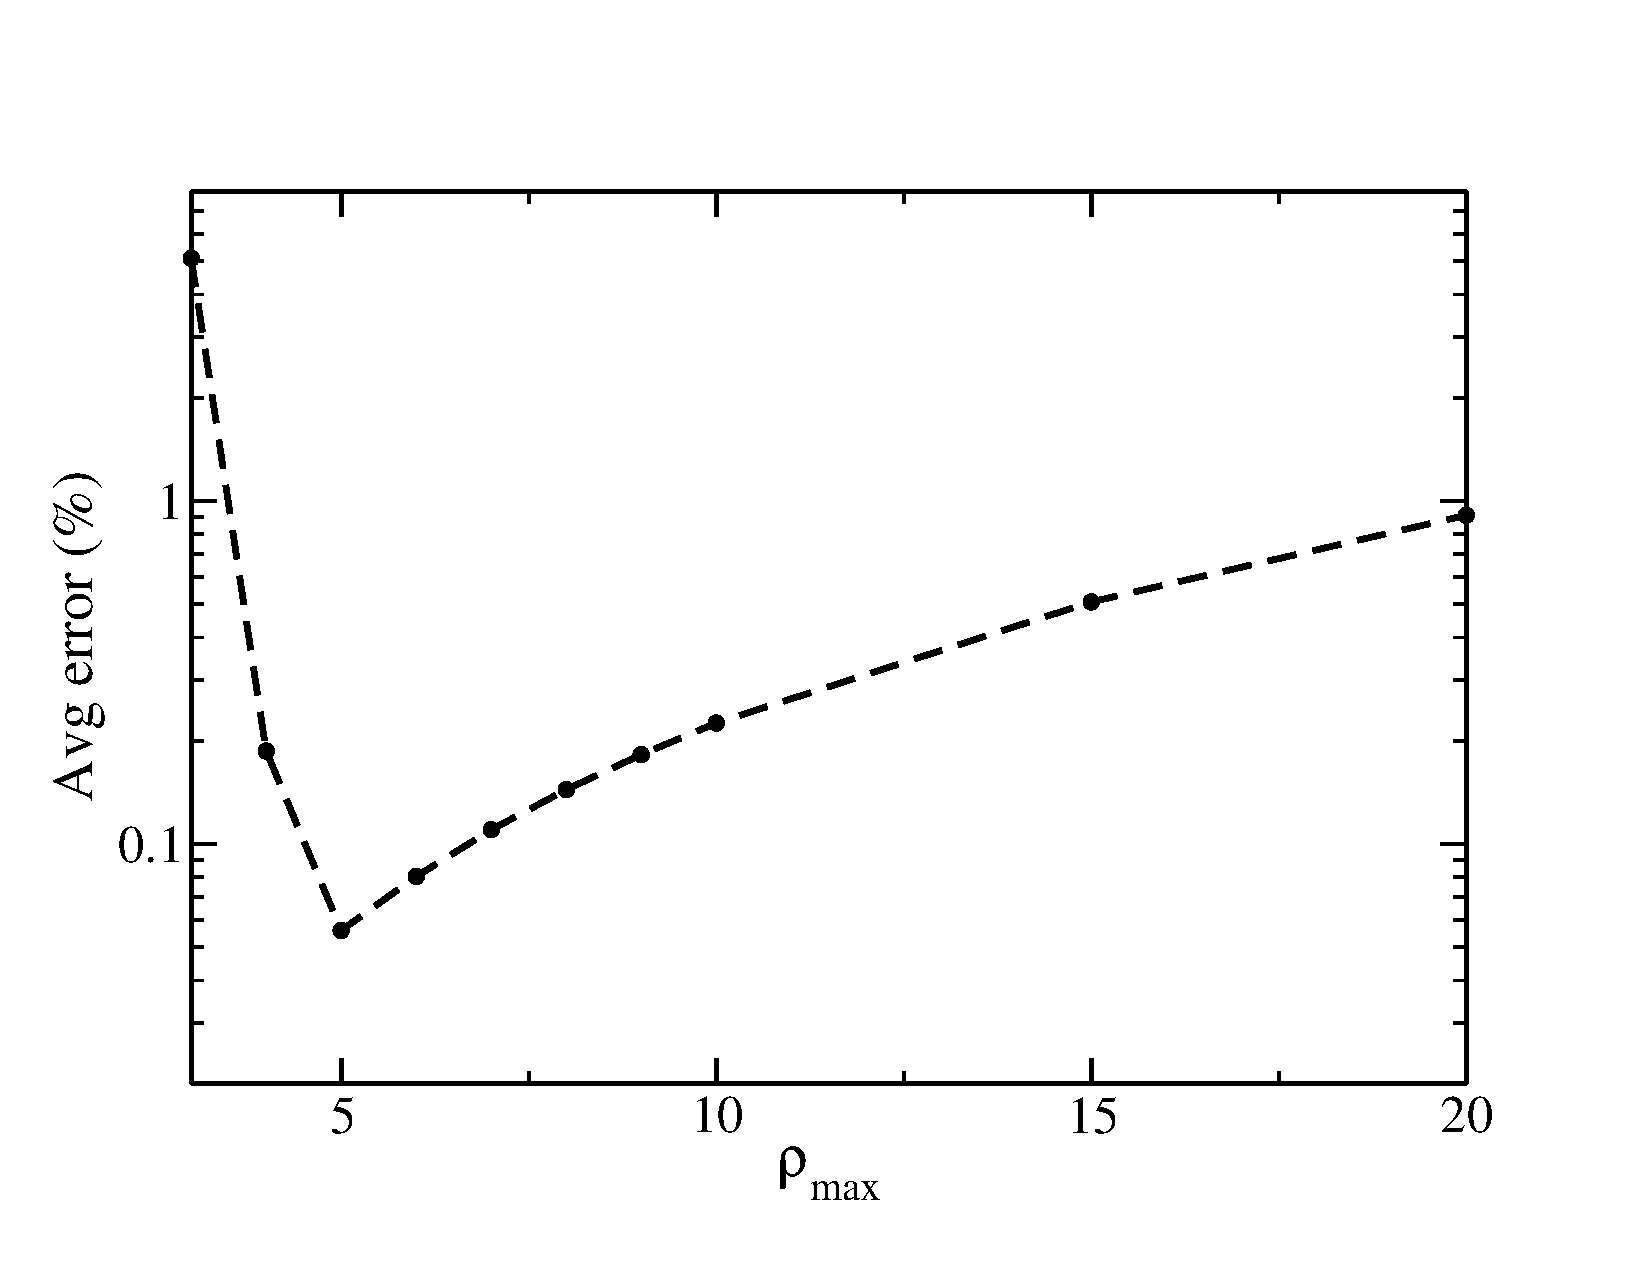
\includegraphics[scale=0.33]{error_pmax.pdf}
\caption{Relative average error in $\lambda_n$ as a function of $\rho_{max}$}
\label{err}
\end{figure}

In addition, we test the performance of the code via the CPU time to solution for varying matrix dimension. In Figure~\ref{arma}, we compare the performance of our Jacobi algorithm (black solid curve) to that of a more sophisticated algorithm (red dashed curve) from the Armadillo library~\cite{armadillo}. 

In general, one would expect the Armadillo algorithm to be faster regardless of matrix size; however, for very small matrix dimension, the Jacobi algorithm is faster. This is likely because the value of $\rho_{max}$ was kept constant and only the matrix dimension was changed. This means that for the small matrix sizes, the step size was larger, which means the off-diagonal matrix elements (which go like $1/h^2$) are smaller. For the values plotted in Figure~\ref{arma}, $\rho_{max}$ = 10, which means for matrices under $N=10$ the off diagonal elements would be less than 1, while for matrices around $N=100$ the off diagonal elements would be closer to 100. This means that not only do there need to be more iterations for larger matrices because of the %are %more values, but the values will also be much further from zero. 

\begin{table}[b]
\centering
\begin{tabular}{|c|c|c|c|c|}
\hline
$\lambda_n$&Jacobi & Analytic & Jacobi & Analytic\\
\hline
$\lambda_0$&2.9992&3&0.3499&0.35\\
$\lambda_1$&6.9961&7&0.5325&N/A\\
$\lambda_2$&10.9906&11&0.7210&N/A\\
\hline
\end{tabular}
\caption{Comparison of eigenvalues for the analytic methods and the Jacobi method. For the non-interacting case N = 100 and $\rho_{max}$=5. For the interacting case N = 200$\rho_{max}=20$ and $\omega_r$ = 0.05. Analytic values for the interacting case are from~\cite{interact}.}
\label{eigen}
\end{table}

\begin{figure}[t]
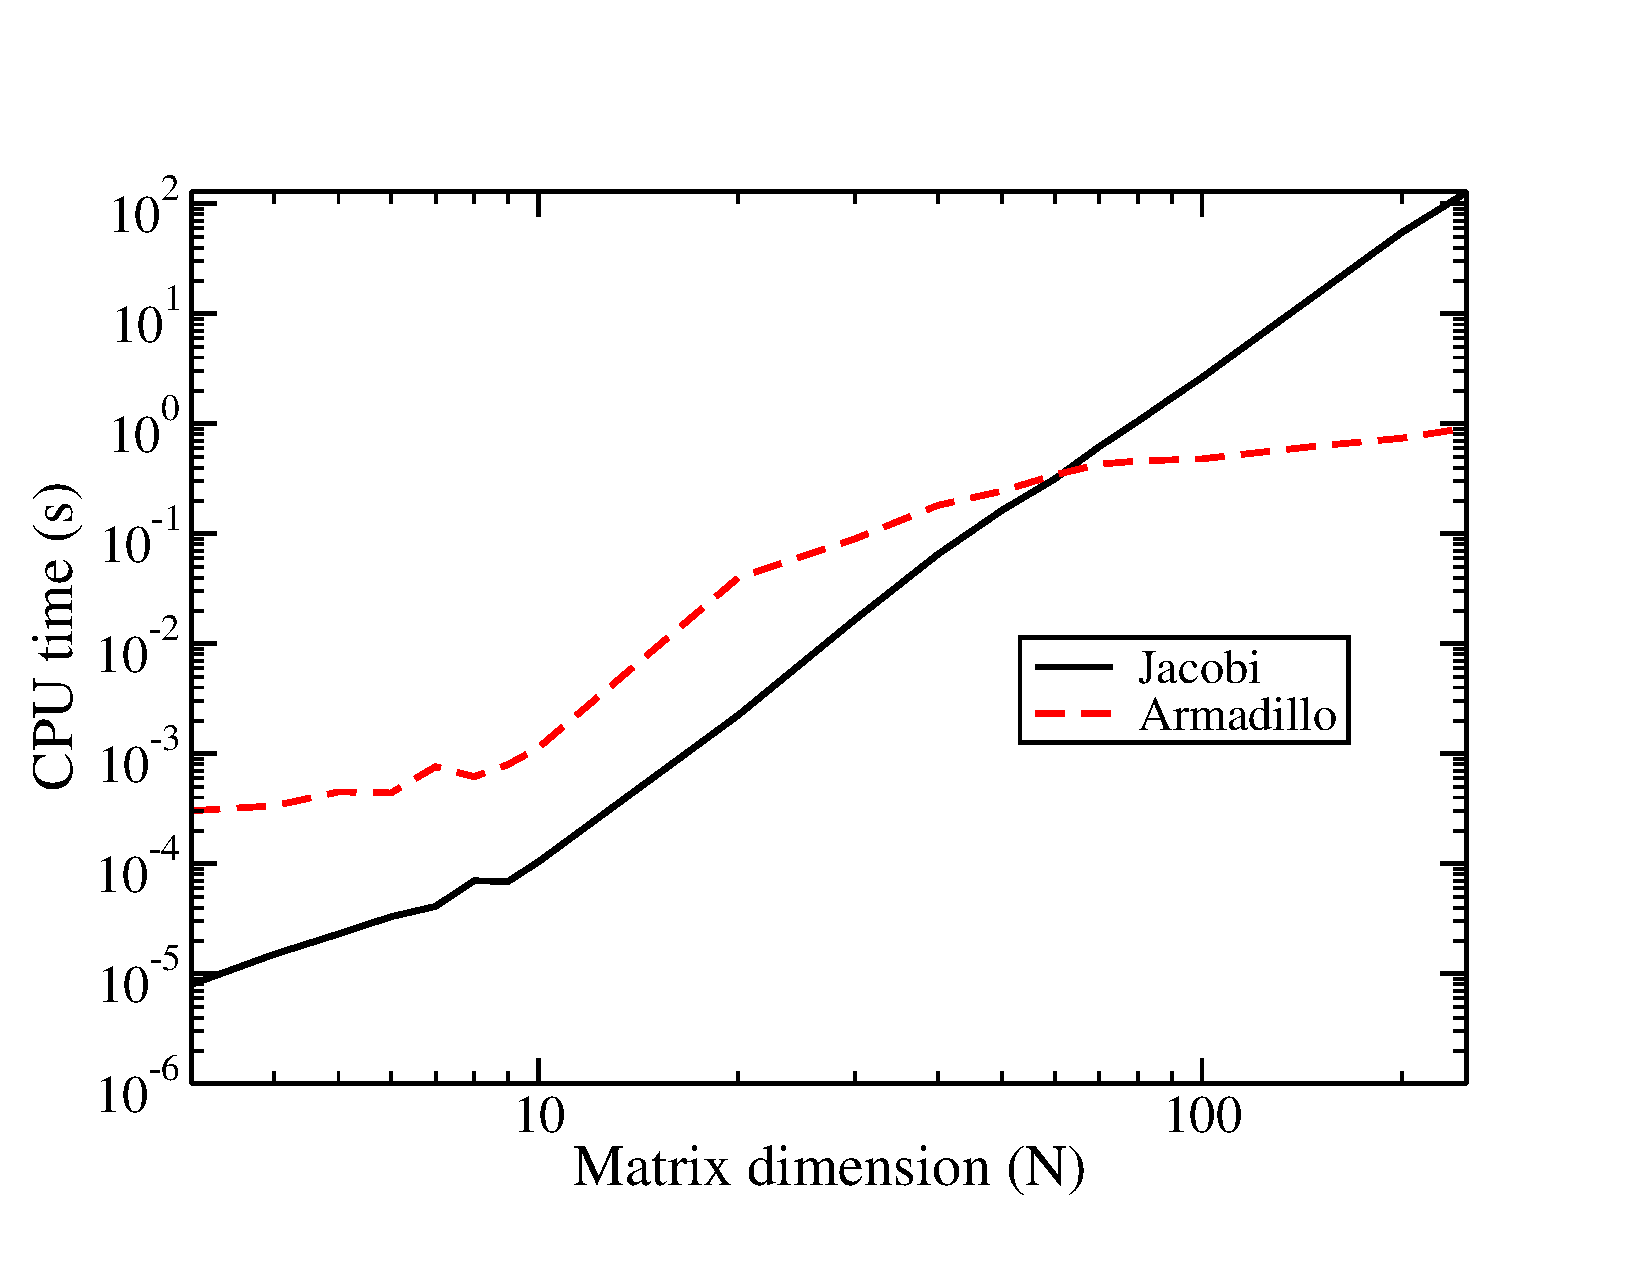
\includegraphics[scale=0.33]{N_time2.pdf}
\caption{Computation time as a function of matrix dimension.}
\label{arma}
\end{figure}

\noindent larger number of values, but the values will also be much further from zero. 

This point is further illustrated in Figure~\ref{trans}, which shows the number of Jacobi rotations needed for the off diagonal elements to be less than 0.001. The black solid line corresponds to the results from the Jacobi algorithm, and the red dashed line corresponds to the predicted behavior. We expect the number of iterations should scale as $N^2$ because the number of matrix elements to transform scales as $N^2$. For large matrices the results agree well with the prediction, but for small matrices the Jacobi algorithm needs less iterations than expected. Again, this is likely due to the small size of the off diagonal matrix elements for small matrix sizes.

\begin{figure}[b]
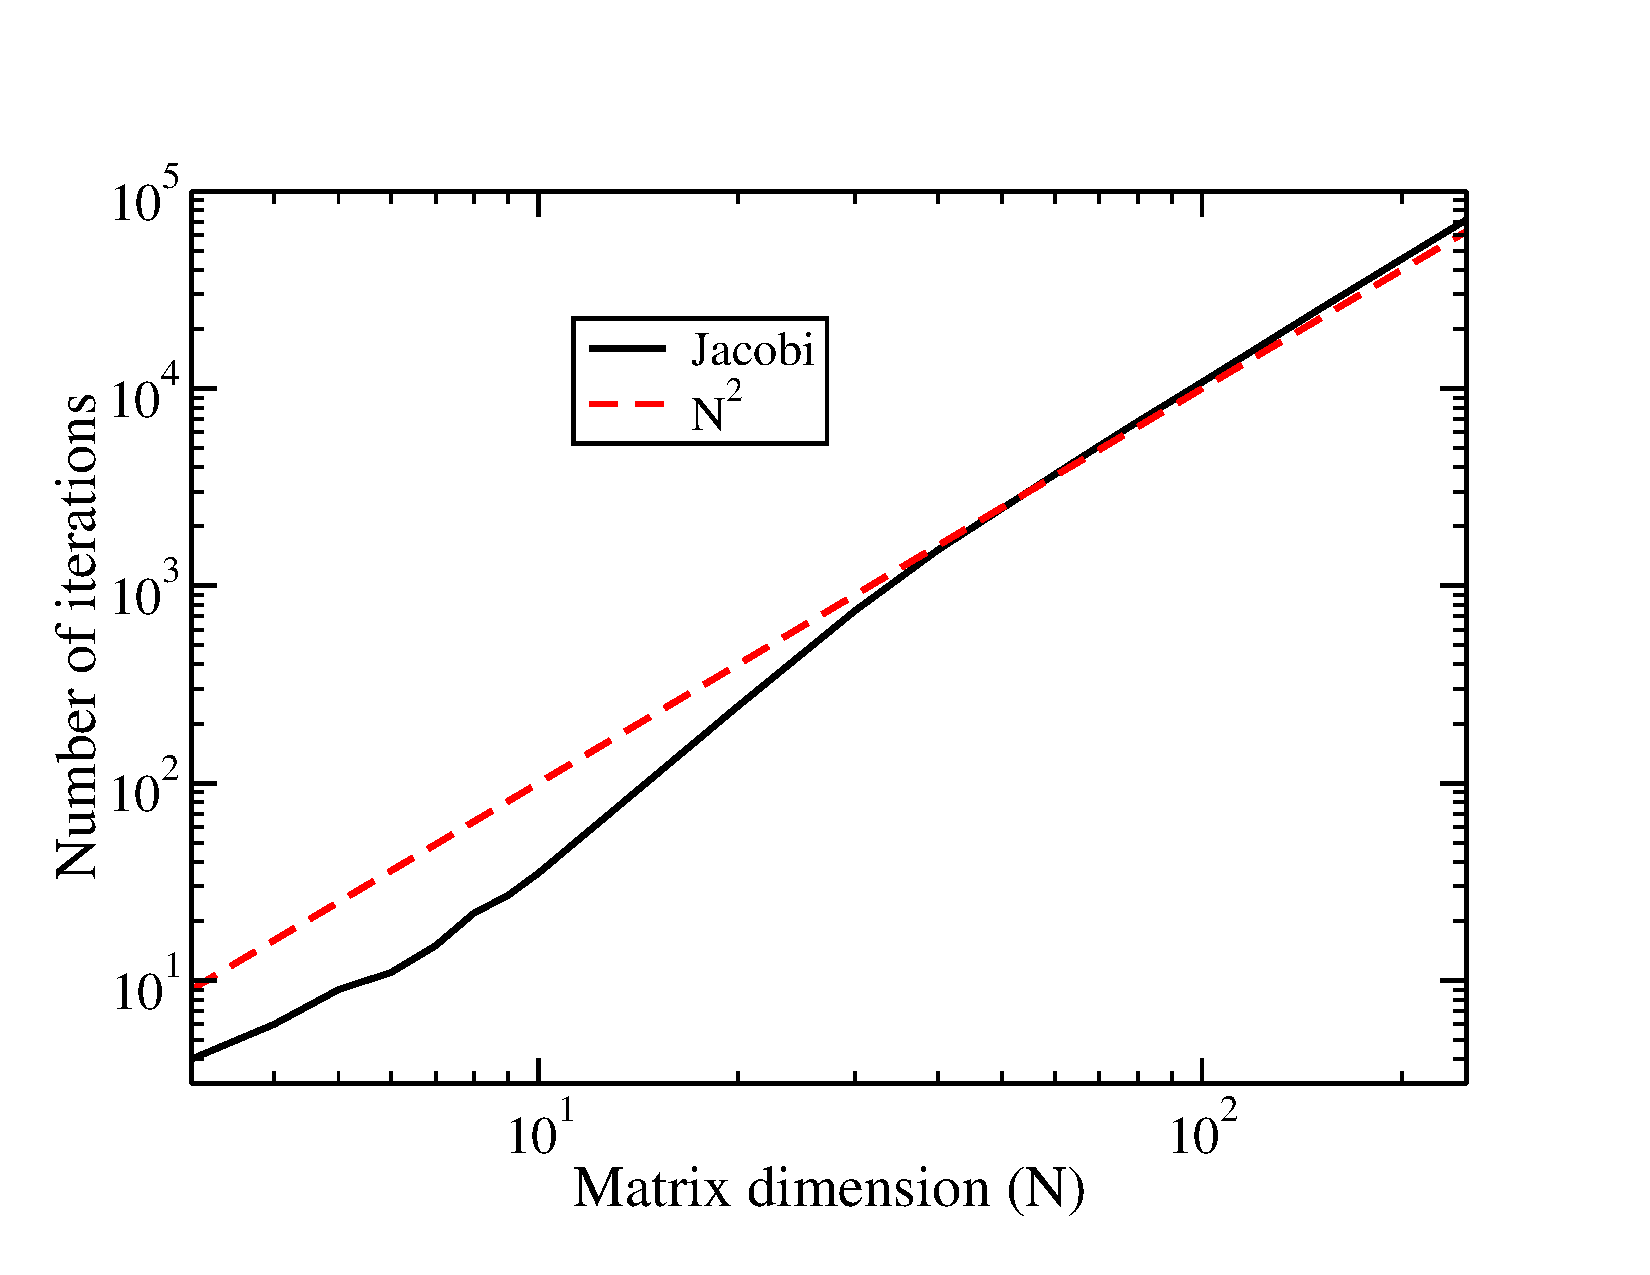
\includegraphics[scale=0.33]{N_trans.pdf}
\caption{Number of Jacobi rotations necessary for convergence as a function of matrix dimension.}
\label{trans}
\end{figure}

\begin{figure}[t]
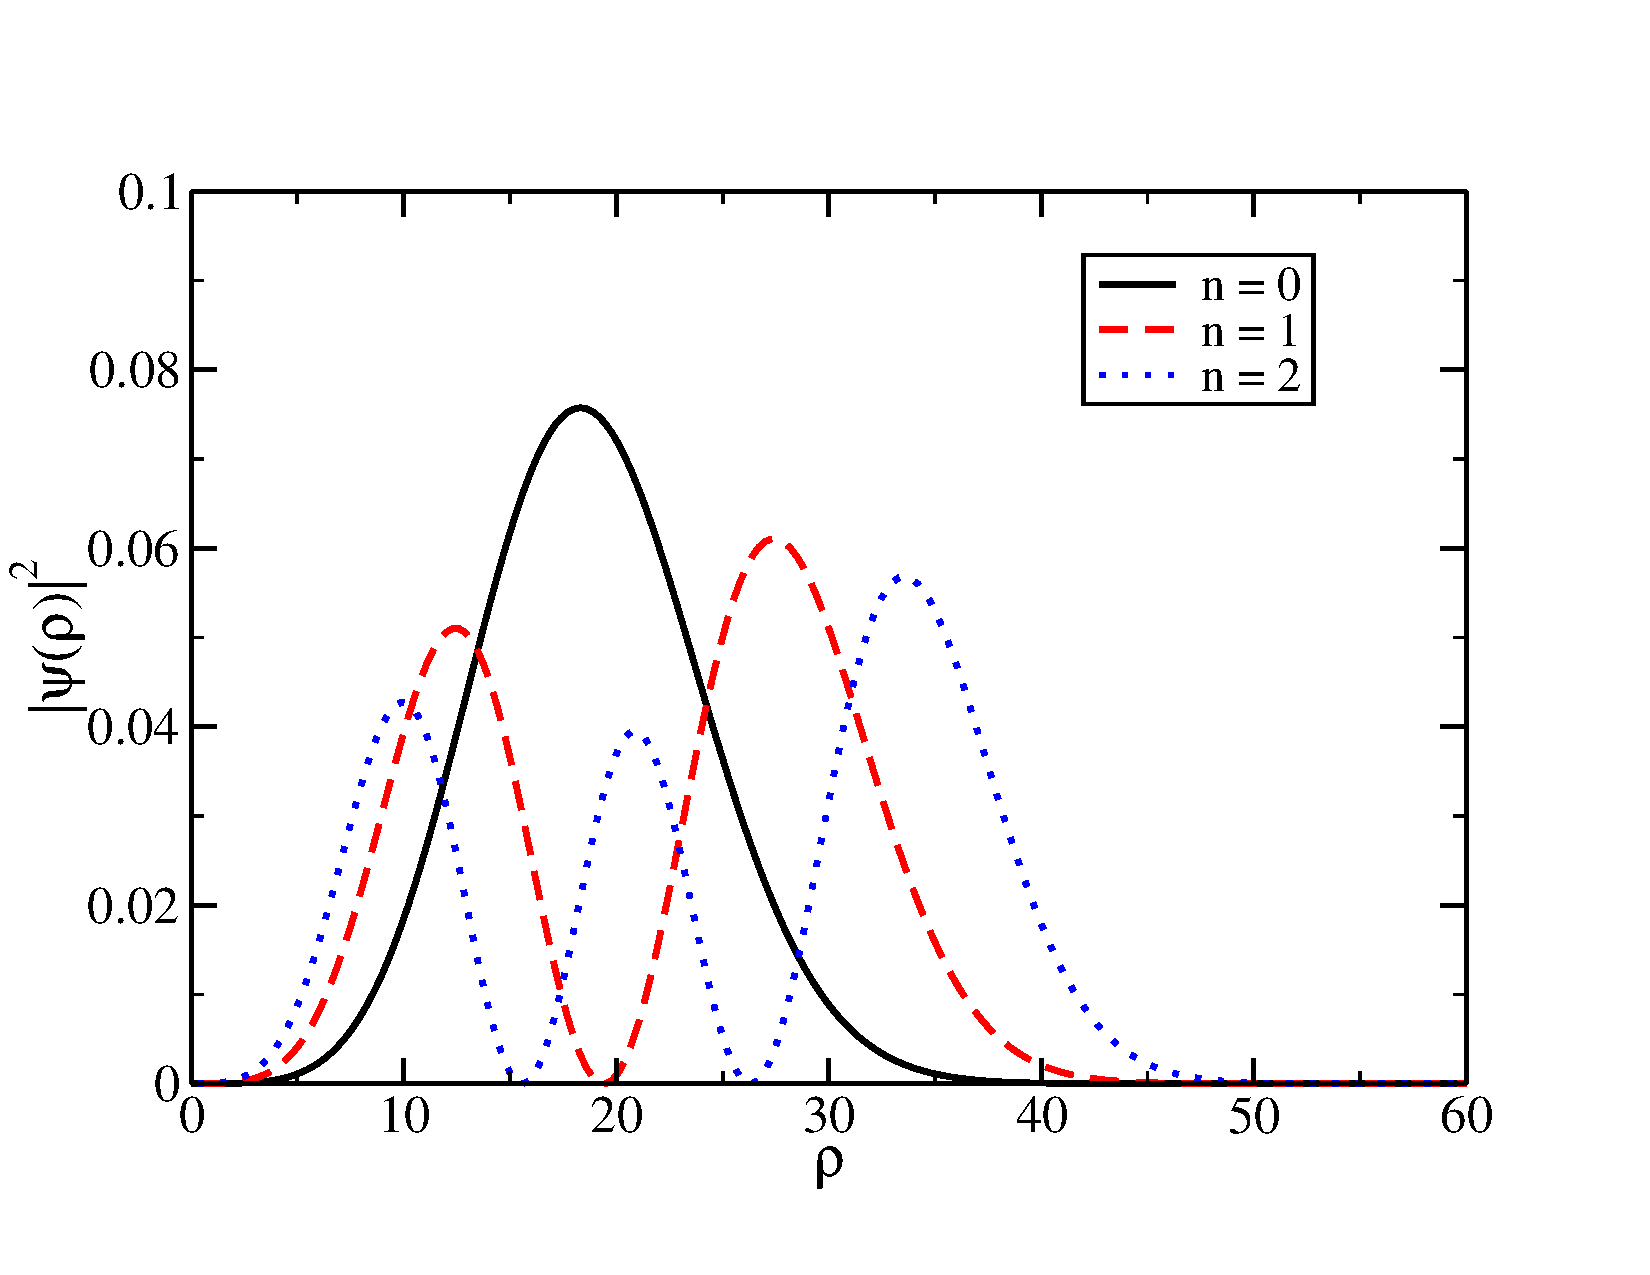
\includegraphics[scale=0.33]{wf_01.pdf}
\caption{$|\psi(\rho)|^2$ for $w_r = 0.01$}
\label{wf_01}
\end{figure}

\subsection{Interacting Case}
We now implement the Jacobi algorithm with the harmonic oscillator potential and a Coulomb interaction potential. First, we use the oscillator frequency of $\omega_r=0.05$ from~\cite{interact} and compare their eigenvalues to those calculated with the Jacobi algorithm in Table~\ref{eigen}. Again, there is good agreement with the analytic solution.

In addition, we compare the probability distribution of the wave functions, $|\psi_n(\rho)|^2$, for varying $\omega_r$ in Figures~\ref{wf_01}-\ref{wf_5}. In all figures the black solid line corresponds to the ground state, and the red dashed (blue dotted) line corresponds to the first (second) excited state. Figure~\ref{wf_01} shows the distribution for $\omega_r$ = 0.01, Figure~\ref{wf_05} for $\omega_r = 0.05$, Figure~\ref{wf_1} for $\omega_r = 1.0$, and Figure~\ref{wf_5} for $\omega_r = 5.0$.

\begin{figure}[b]
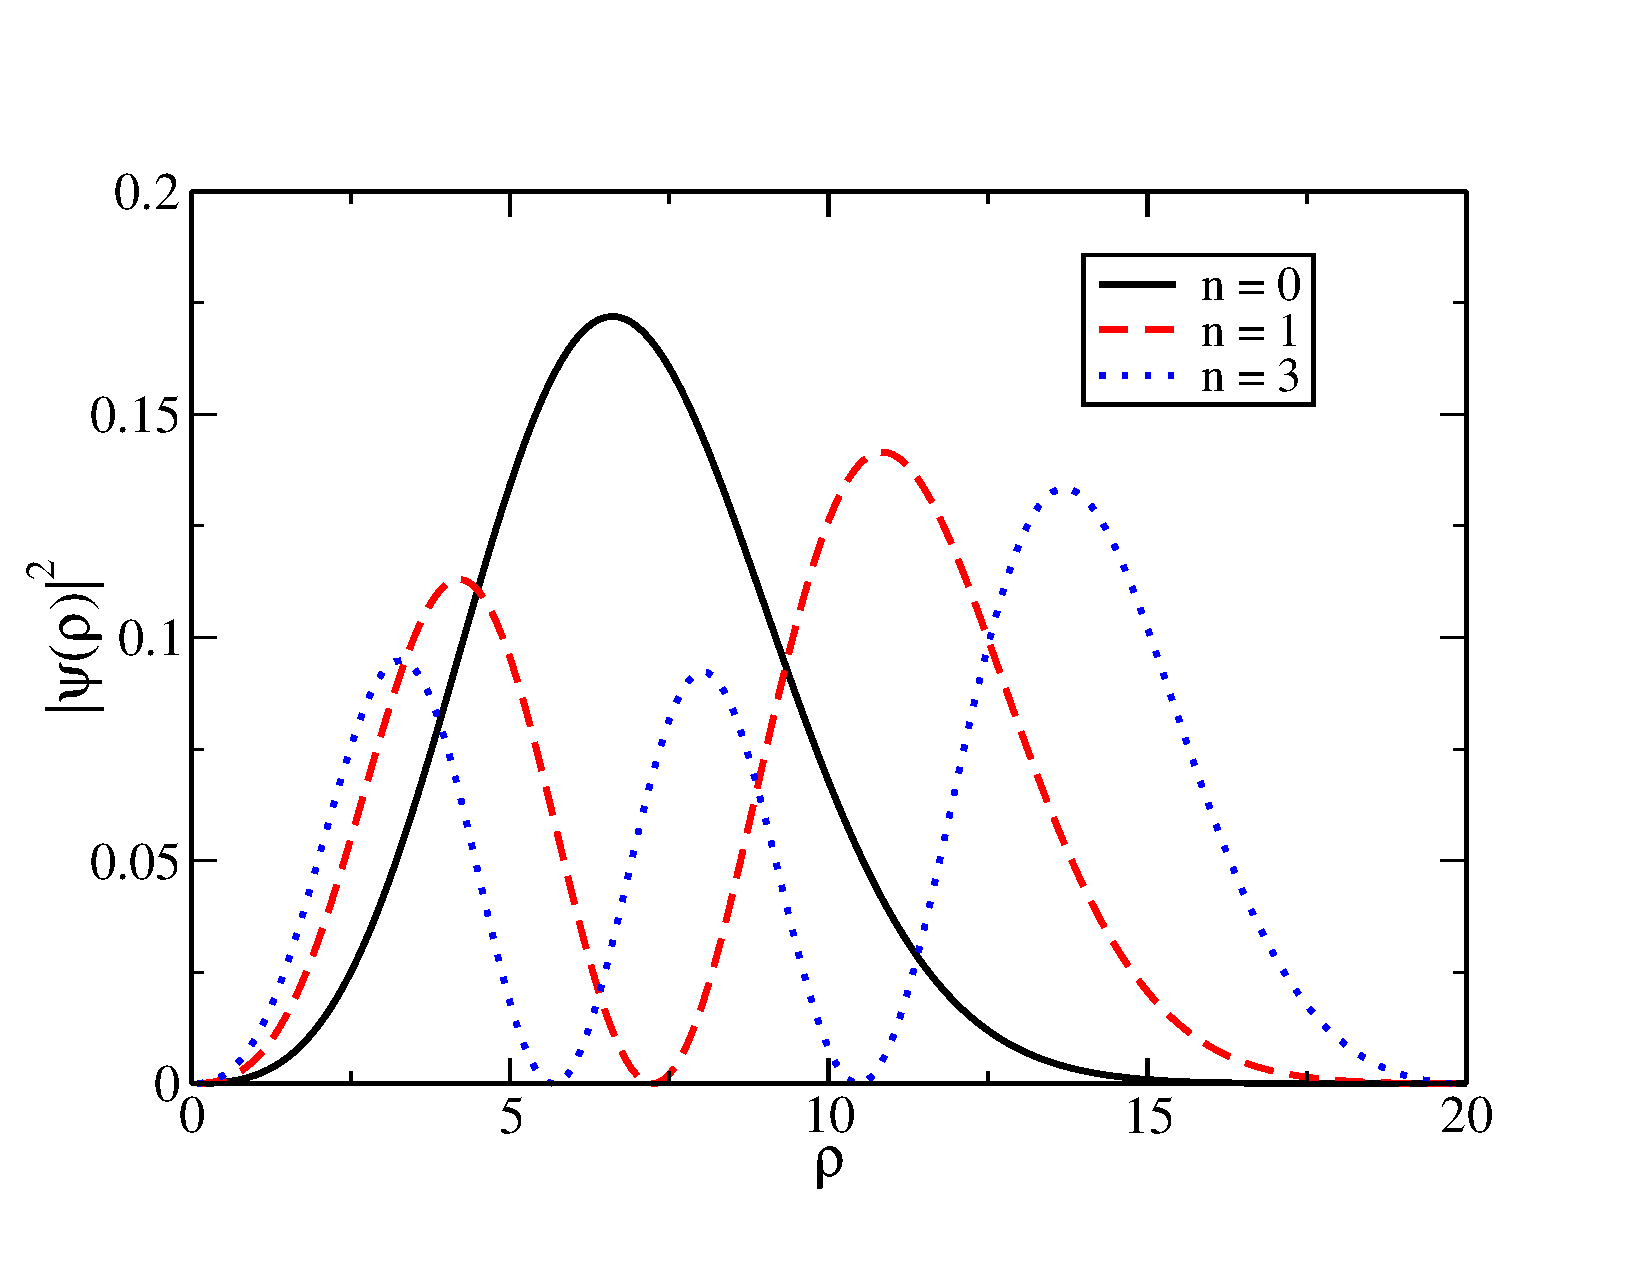
\includegraphics[scale=0.33]{wf_05.pdf}
\caption{$|\psi_n(\rho)|^2$ for $w_r = 0.05$}
\label{wf_05}
\end{figure}

\begin{figure}[t]
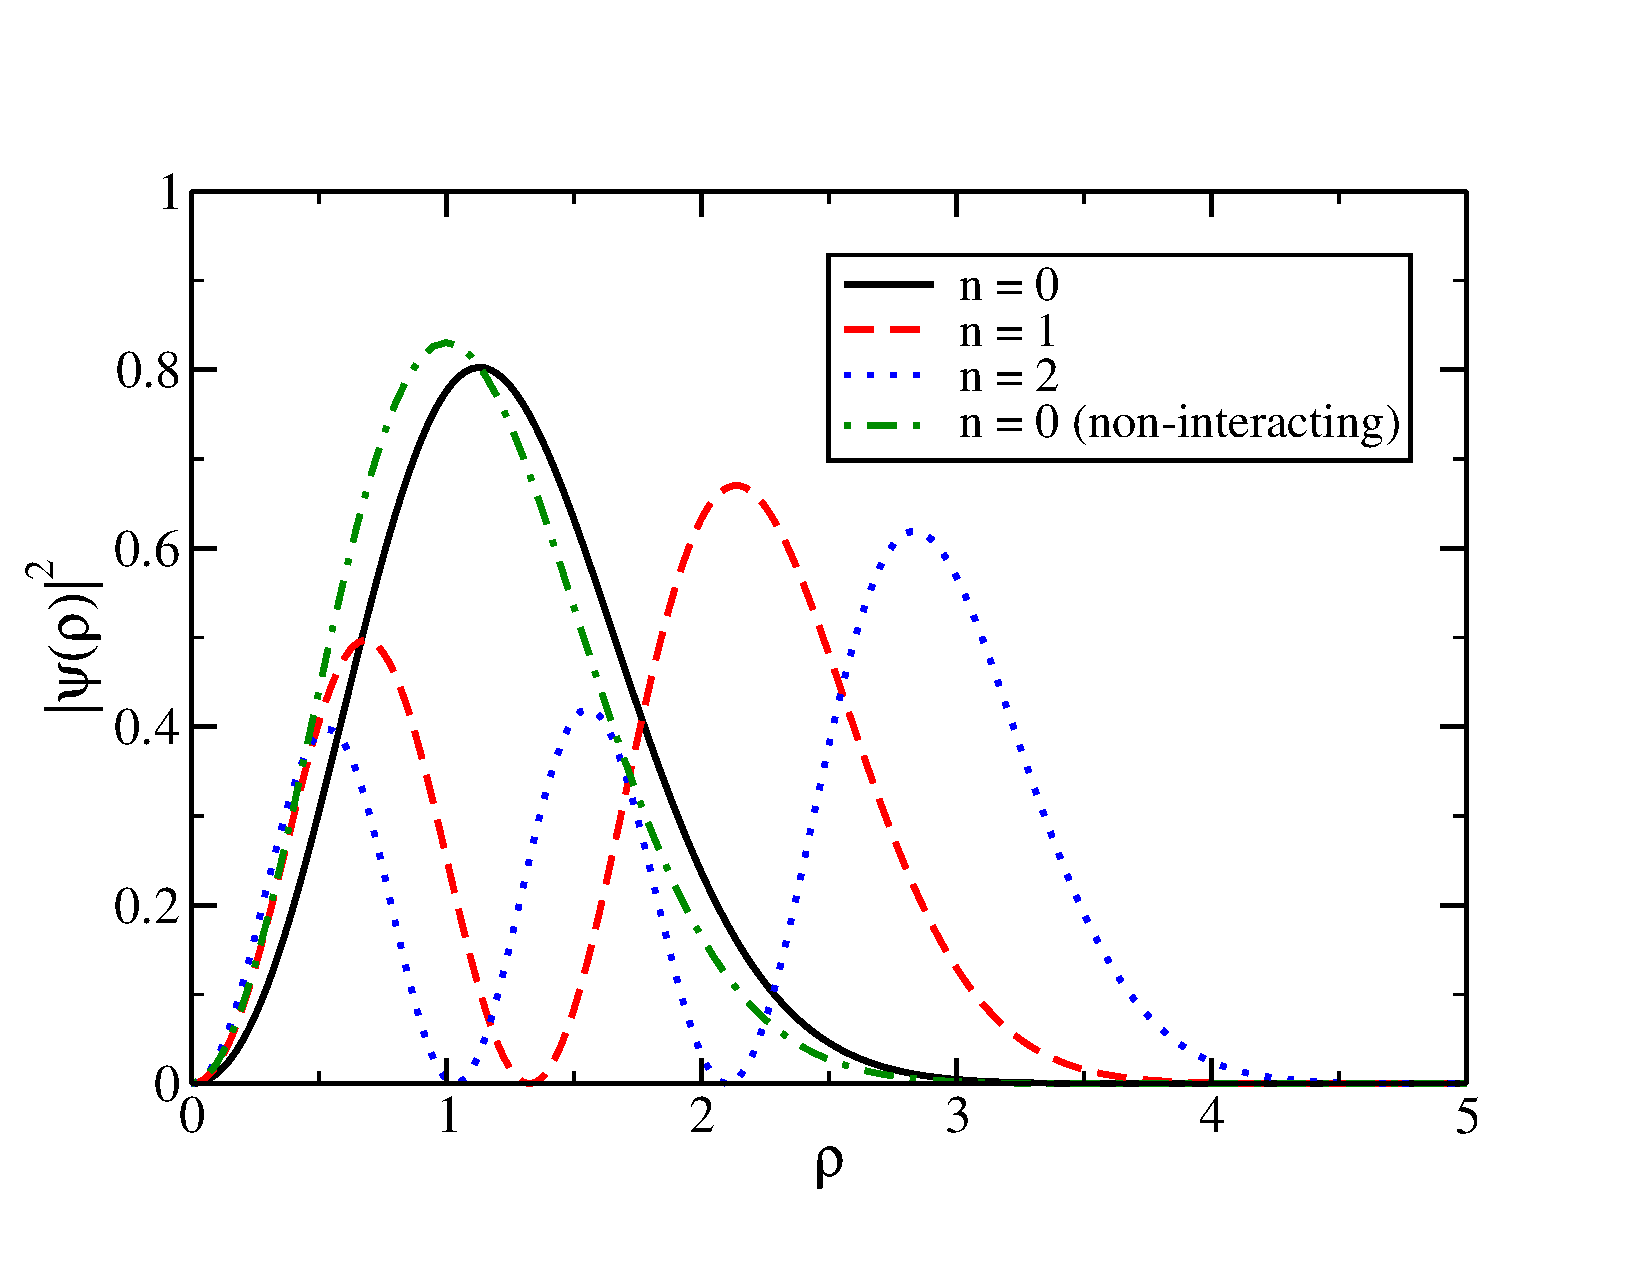
\includegraphics[scale=0.33]{wf_1.pdf}
\caption{$|\psi_n(\rho)|^2$ for $w_r = 1.0$}
\label{wf_1}
\end{figure}

As $\omega_r$ represents the strength of the harmonic oscillator potential, as $\omega_r$ increases, there should be less space for the two electrons and thus the probability distribution should be peaked at smaller values of $\rho$. This is indeed the same behavior seen in Figures~\ref{wf_01}-\ref{wf_5} as the peak for the ground state probability distribution moves from roughly $\rho=20$ for $\omega_r=0.01$ to under 0.5 for $\omega_r=5.0$

Finally, in Figure~\ref{wf_1} we show the ground state wave function probability distribution with no coulomb interaction (green dot-dashed line) for comparison. Here we can see that the inclusion of the Coulomb repulsion causes the probability distribution to be shifter to larger $\rho$ and more diffuse. This is to be expected as the Coulomb repulsion causes the the two electrons to be pushed away from one another.

\begin{figure}[b]
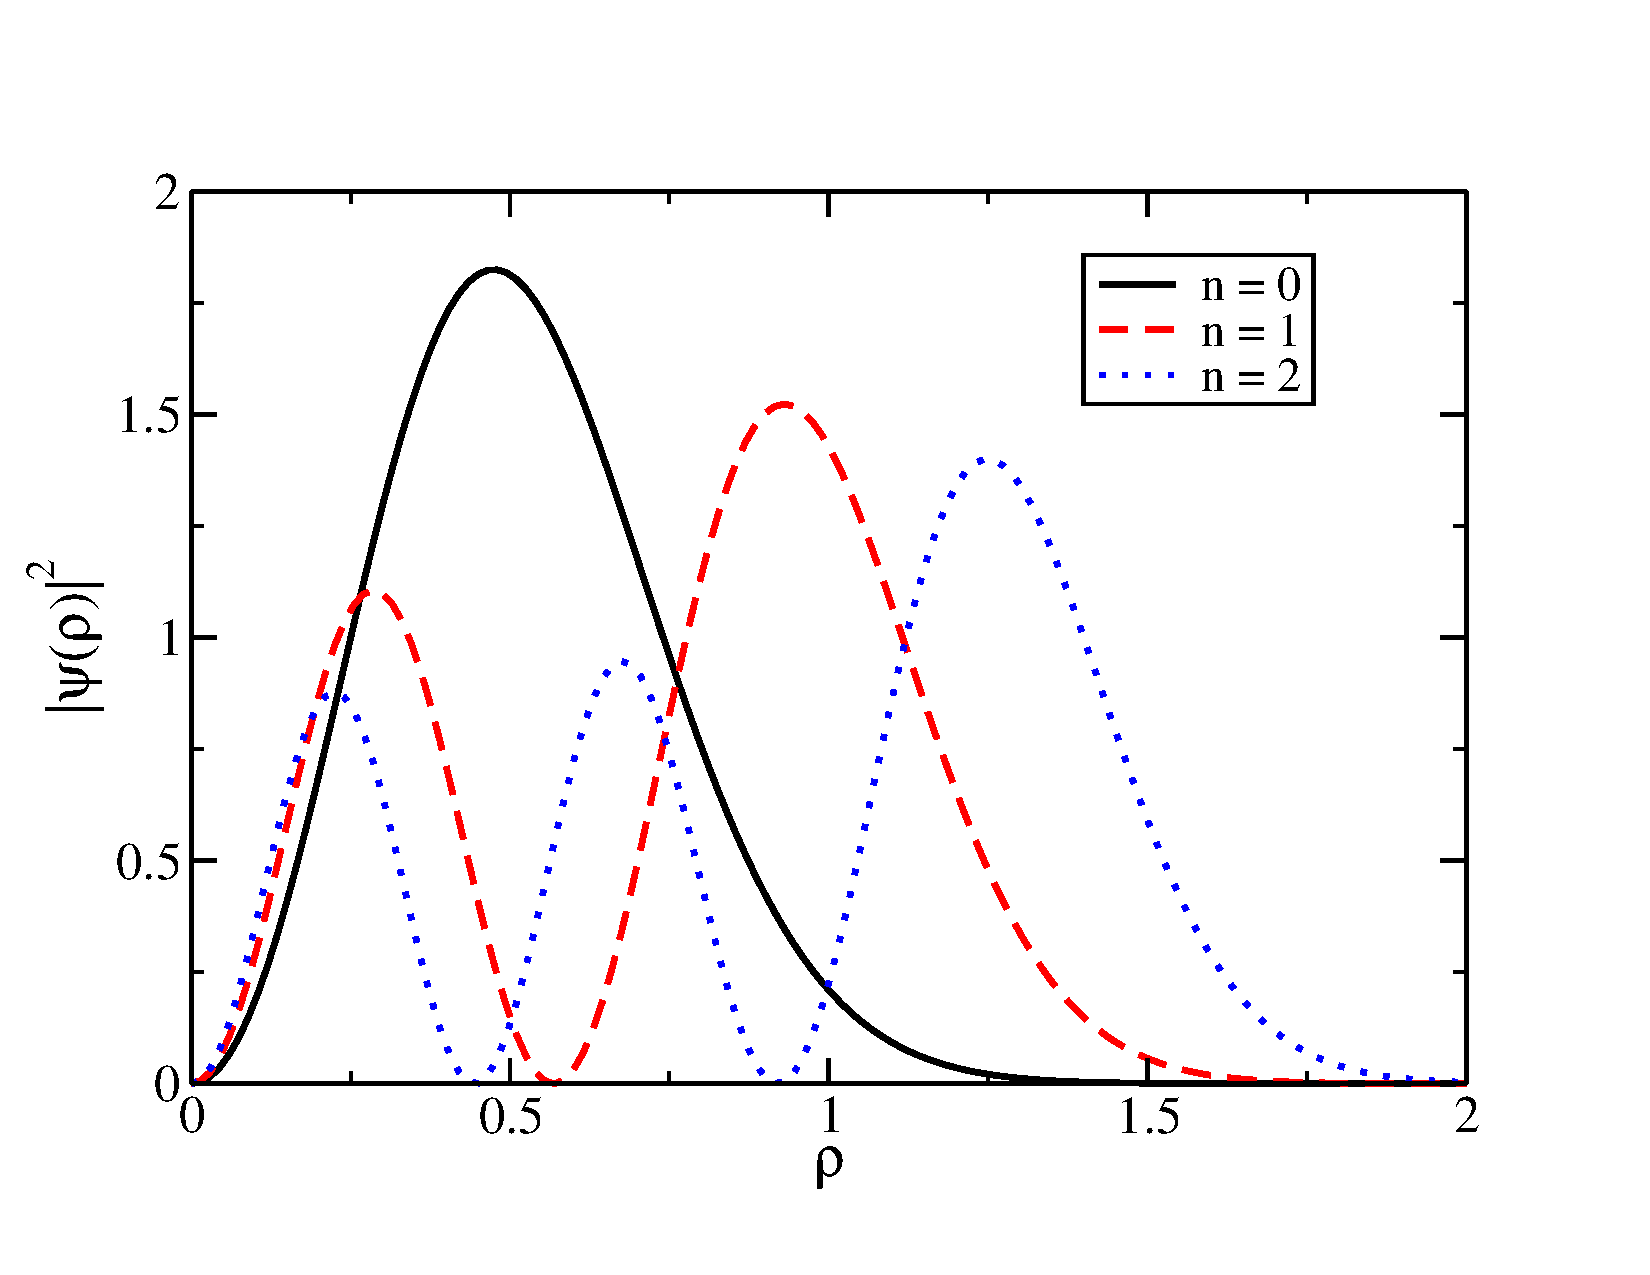
\includegraphics[scale=0.33]{wf_5.pdf}
\caption{$|\psi_n(\rho)|^2$ for $w_r = 5.0$}
\label{wf_5}
\end{figure}

\section{conclusions}
\label{conc}

\bibliography{jacobi}
\end{document}

